\documentclass[10pt]{beamer}

\usepackage[english]{babel}
\usepackage[utf8]{inputenc}
\usepackage{amsmath,amssymb,amsthm,latexsym}
\usepackage{mathrsfs}
\usepackage[all]{xypic}
\usepackage{tikz}
\usetikzlibrary{arrows,shapes,automata}
\usepackage{eurosym}
\usepackage{listings}
\usepackage{textcomp}
\usepackage{soul}

\newcommand{\cat}[1]{\mathscr{#1}}
\newcommand{\lcat}[1]{\mathbf{#1}}
\renewcommand{\L}{\cat{L}}
\newcommand{\comp}{\circ}
\newcommand{\size}[1]{\lVert#1\rVert}
\newcommand{\sizein}[1]{\size{#1}^\mathrm{in}}
\newcommand{\sizeout}[1]{\size{#1}_\mathrm{out}}
\DeclareMathOperator{\ob}{ob}
\DeclareMathOperator{\Hom}{Hom}
\DeclareMathOperator{\id}{id}
\DeclareMathOperator{\Id}{Id}
\newcommand{\N}{\mathbb{N}}
\newcommand{\Z}{\mathbb{Z}}
\newcommand{\C}{\mathbb{C}}
\newcommand{\R}{\mathbb{R}}
\newcommand{\K}{\mathbb{K}}
\newcommand{\LK}{\mathbb{L}}
\newcommand{\ra}{\rightarrow}
\newcommand{\la}{\leftarrow}
\DeclareMathOperator{\Time}{t}
\DeclareMathOperator{\Space}{s}
\DeclareMathOperator{\coTime}{co-t}
\DeclareMathOperator{\coSpace}{co-s}
\DeclareMathOperator{\Par}{Par}
\DeclareMathOperator{\Tr}{Tr}
\DeclareMathOperator{\rev}{rev}
\newcommand{\computes}{\vdash}
\renewcommand{\u}{\underline}
\renewcommand{\o}{\overline}
\newcommand{\tALpy}{\texttt{transalpyne}}

\newenvironment{pictureframe}{
  \addtocounter{framenumber}{-1}
  \setbeamertemplate{navigation symbols}{}
  \setbeamercolor{background canvas}{bg=black}
  \begin{frame}[plain,fragile,environment=pictureframe]%
    \begin{center}%
    }{%
    \end{center}%
  \end{frame}%
}

\lstset{
  language=haskell,
  upquote=true,
  basicstyle=\ttfamily,          % print whole listing in typewriter
  keywordstyle=\color{blue}\bfseries, % bold blue keywords
  %identifierstyle=,           % nothing happens
  commentstyle=\color{green}, % green comments
  stringstyle=\color{red},      % typewriter type for strings
  showstringspaces=false     % no special string spaces
}


\mode<presentation>{%
  \usetheme[]{Madrid}
  \usecolortheme{seahorse}
  \usecolortheme{rose}
  \usefonttheme[onlymath]{serif}
}


\title{\tALpy{}: a language for automatic transposition}
\author[\textbf{L. De Feo} and
É.~Schost]{\textbf{L.~De~Feo}\footnotemark and
  É.~Schost\footnotemark\\{(part of this talk is joint work with
    M. Boespflug\footnotemark[1])}} \institute[X and
UWO]{\footnotemark[1]LIX, École Polytechnique\\\footnotemark[2]SCL,
  University of Western Ontario} \date[Paris, July 8, 2010]{PLMMS
  @CICM 2010\\Conservatoire National des Arts et Métiers\\Paris, July
  8, 2010}

% \AtBeginSection[]
% {
%   \begin{frame}<beamer>
%     \frametitle{Plan}
%     \tableofcontents[currentsection]
%   \end{frame}
% }


\begin{document}

\begin{frame}
  \titlepage
\end{frame}

%%
%%

\begin{frame}
  \frametitle{Or, ``The day I discovered I suffer from schizophrenia''}

  \begin{columns}[c]
    \begin{column}{0.5\textwidth}
      \begin{center}
        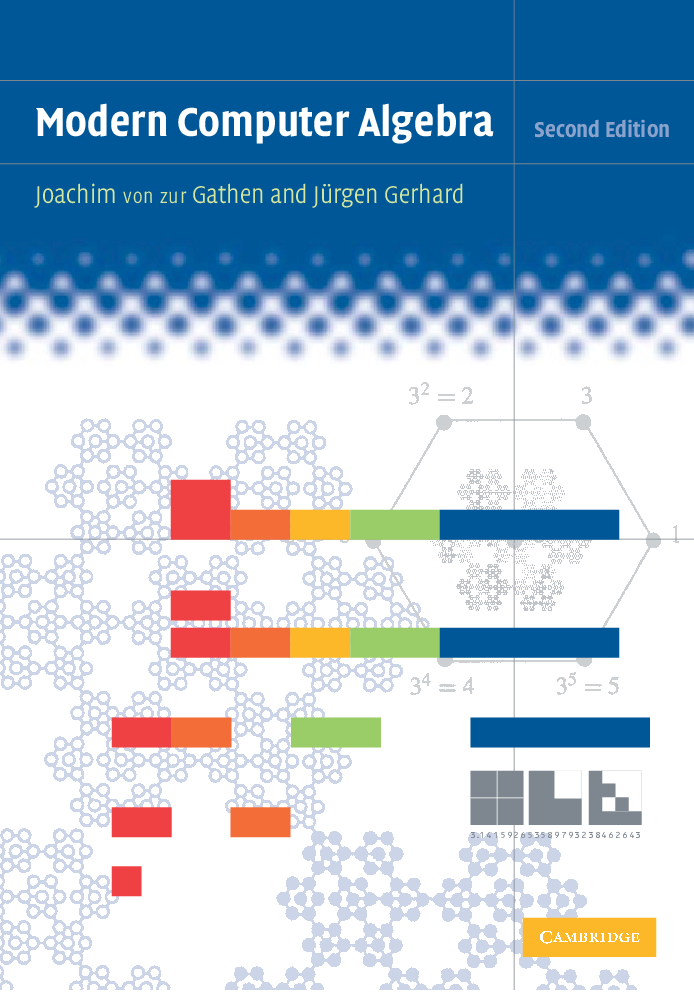
\includegraphics[width=0.8\textwidth]{modern.png}

        %$\xymatrix{&&&\\\ar[ur]}$

        Mr. Jekyll is a computer algebraist\\
        (he'll eventually become Dr.)
      \end{center}
    \end{column}
    \begin{column}{0.5\textwidth}
      \begin{center}
        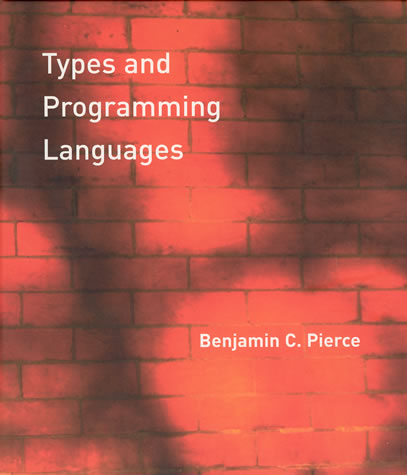
\includegraphics[width=0.8\textwidth]{types.jpg}
        
        % $\xymatrix{&&&\\&&&\ar[ul]}$

        Mr Type wastes precious time committed to thesis writing, by
        reading about types and categorical semantics
      \end{center}
    \end{column}
  \end{columns}
\end{frame}

%%

\begin{pictureframe}
  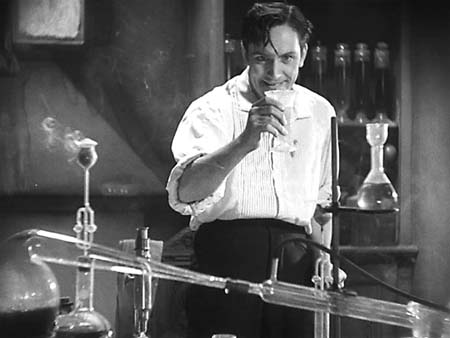
\includegraphics[width=\textwidth]{jekyll1}
\end{pictureframe}

%%
%%

\section{The transposition principle}

\begin{frame}
  \frametitle{Matrices represented by computer programs?!}

  \begin{block}{The black box model}
    If $A$ is a sparse or structured matrix, it is cheaper to restrict
    to algorithms that only query a black box:
    \[\xymatrix{
      b\ar[r]  & \rule{10ex}{2em} \ar[r] & A\cdot b
    }\]
  \end{block}
  
  \begin{block}{Applications}
    \begin{itemize}
    \item The good ol' \alert{Power iteration method} to find the
      largest eigenvalue. Used by Google page ranking algorithm
      \cite{google}.
    \item Wiedemann's algorithms for minimal/characteristic
      polynomial, determinant, rank, inversion. \cite{Wie86}
    \item \dots
    \end{itemize}
  \end{block}
\end{frame}

%%

\begin{frame}
  \frametitle{Arithmetic circuits}

  \begin{columns}
    \begin{column}{0.6\textwidth}
      \centering
      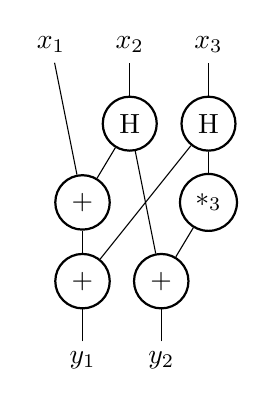
\begin{tikzpicture}
        \tikzstyle{node}=[circle,thick,draw=black,minimum size=4mm]
        
        \begin{scope}
          \node(x1){$x_1$};
          \node(x2)[right of=x1]{$x_2$};
          \node(x3)[right of=x2]{$x_3$};
          
          \node[node](d1)[below of=x2]{H}
          edge(x2);
          \node[node](d2)[below of=x3]{H}
          edge(x3);
          
          \node[node](p1)[below of=d1,xshift=-6mm]{$+$}
          edge(x1)
          edge(d1);
          \node[node](m1)[below of=d2]{$*_3$}
          edge(d2);
          
          \node[node](p2)[below of=p1]{$+$}
          edge(p1)
          edge(d2);
          \node[node](p3)[right of=p2]{$+$}
          edge(d1)
          edge(m1);
          
          \node(y1)[below of=p2]{$y_1$}
          edge(p2);
          \node(y2)[below of=p3]{$y_2$}
          edge(p3);
        \end{scope}
      \end{tikzpicture}
    \end{column}
    \begin{column}{0.4\textwidth}
      \begin{align*}
        y_1 &= x_1 + x_2 + x_3\\
        y_2 &= x_2 + 3x_3
      \end{align*}
      
      \Large
      \begin{gather*}
        \begin{pmatrix}
          1 & 1 & 1\\
          0 & 1 & 3
        \end{pmatrix}
      \end{gather*}
    \end{column}
  \end{columns}
\end{frame}

%%

\begin{frame}
  \frametitle{Transposition of an arithmetic circuit}

  \begin{columns}
    \begin{column}{0.6\textwidth}
      \centering
      \begin{tikzpicture}
        \tikzstyle{node}=[circle,thick,draw=black,minimum size=4mm]
        
        \begin{scope}
          \node(x1){$x_1$};
          \node(x2)[right of=x1]{$x_2$};
          \node(x3)[right of=x2]{$x_3$};
          
          \node[node](d1)[below of=x2]{H}
          edge(x2);
          \node[node](d2)[below of=x3]{H}
          edge(x3);
            
          \node[node](p1)[below of=d1,xshift=-6mm]{$+$}
          edge(x1)
          edge(d1);
          \node[node](m1)[below of=d2]{$*_3$}
          edge(d2);
          
          \node[node](p2)[below of=p1]{$+$}
          edge(p1)
          edge(d2);
          \node[node](p3)[right of=p2]{$+$}
          edge(d1)
          edge(m1);
          
          \node(y1)[below of=p2]{$y_1$}
          edge(p2);
          \node(y2)[below of=p3]{$y_2$}
          edge(p3);
        \end{scope}
        
        \begin{scope}[xshift=3.2cm, yshift=-0.23\textheight]
          \node(x){\Huge $\leftrightarrow$};
        \end{scope}
        
        \begin{scope}[xshift=4cm, yshift=-0.425\textheight]
          \node(x1){$x_1'$};
          \node(x2)[right of=x1]{$x_2'$};
          \node(x3)[right of=x2]{$x_3'$};
          
          \node[node](d1)[above of=x2]{\alt<2>{$+$}{H}}
          edge(x2);
          \node[node](d2)[above of=x3]{\alt<2>{$+$}{H}}
          edge(x3);
          
          \node[node](p1)[above of=d1,xshift=-5mm]{\alt<2>{H}{$+$}}
          edge(x1)
          edge(d1);
          \node[node](m1)[above of=d2]{$*_3$}
          edge(d2);
          
          \node[node](p2)[above of=p1]{\alt<2>{H}{$+$}}
          edge(p1)
          edge(d2);
          \node[node](p3)[right of=p2]{\alt<2>{H}{$+$}}
          edge(d1)
          edge(m1);
          
          \node(y1)[above of=p2]{$y_1'$}
          edge(p2);
          \node(y2)[above of=p3]{$y_2'$}
          edge(p3);
        \end{scope}
      \end{tikzpicture}
    \end{column}
    \begin{column}{0.4\textwidth}
      \begin{align*}
        y_1 &= x_1 + x_2 + x_3\\
        y_2 &= x_2 + 3x_3
      \end{align*}
      
      \Large
      \begin{gather*}
        \begin{pmatrix}
          1 & 1 & 1\\
          0 & 1 & 3
        \end{pmatrix}\\
        \updownarrow\\
        \begin{pmatrix}
          1 & 0\\
          1 & 1\\
          1 & 3\\
        \end{pmatrix}
      \end{gather*}
    \end{column}
  \end{columns}
\end{frame}

%%
%%

\begin{frame}[fragile]
  \frametitle{Transposition of straight line programs}

  \begin{center}
    \large
    Straight line programs $=$ Arithmetic circuits
  \end{center}

  \begin{columns}
    \begin{column}{0.5\textwidth}
      \begin{center}
        \begin{minipage}{0.7\textwidth}
\begin{semiverbatim}
  a[1] = a[0] + a[1]
  a[0] = 0
  a[2] = a[1] + a[2]
  a[1] = 0
  ...
  a[n-1] = a[n-2] + a[n-1]
  a[n-2] = 0
\end{semiverbatim}
        \end{minipage}
      \end{center}
    \end{column}

    \begin{column}{0.5\textwidth}
      \begin{center}
        \begin{minipage}{0.7\textwidth}
\begin{semiverbatim}
  a[n-2] = 0
  a[n-2] = a[n-2] + a[n-1]
  ...
  a[1] = 0
  a[1] = a[1] + a[2]
  a[0] = 0
  a[0] = a[0] + a[1]
\end{semiverbatim}
        \end{minipage}
      \end{center}
    \end{column}
    \end{columns}
  
  \vfill

  \begin{columns}
    \begin{column}{0.5\textwidth}
      \begin{equation*}
        \begin{pmatrix}
          0 & \hdotsfor{3} & 0\\
          \vdots  &  &\vdots&& \vdots \\
          0 & \hdotsfor{3} & 0\\
          1 & \hdotsfor{3} & 1
        \end{pmatrix}
      \end{equation*}
    \end{column}

    \begin{column}{0.5\textwidth}
      \begin{equation*}
        \begin{pmatrix}
          0 & \hdots & 0 & 1\\
          \vdots  &  \cdots & \vdots & \vdots \\
          0 & \hdots & 0 & 1
        \end{pmatrix}
      \end{equation*}
    \end{column}
  \end{columns}
\end{frame}


%%
%%

\section{Motivations}

\begin{frame}
  \frametitle{What is transposition of programs useful for?}

  \begin{columns}
    \begin{column}{0.5\textwidth}
      \begin{center}
        \textbf{Power projection}$:(\K/k)^\ast\ra k[X]^\ast$
        \[\ell \mapsto \sum_{i>0} \ell(\sigma^i) X^i\]
      \end{center}
    \end{column}
    \begin{column}{0.5\textwidth}
      \begin{center}
        \textbf{Modular composition}$:k[X]\ra\K/k$
        \[g\mapsto g(\sigma)\]
      \end{center}
    \end{column}
  \end{columns}

  \begin{block}{Power projection $=$ transposed modular composition}
    \begin{itemize}
    \item Minimal polynomials in towers of extension fields \cite{Sho95}.
    \item Change of order in triangular sets.
    \item Change of order in Artin-Schreier towers \cite{DFS09},
      application to isogeny computation.
    \end{itemize}
  \end{block}

  \begin{block}{Other applications of transposition}
    \begin{itemize}
    \item Generation of irreducible polynomials.
    \item Complexity bounds on evaluation/interpolation.
    \item Reverse mode in automatic differentiation.
    \end{itemize}
  \end{block}
\end{frame}

%%

\begin{frame}[fragile]
  \tiny
  \frametitle{Why \emph{automatic} transposition?}

  \begin{columns}
    \begin{column}{0.5\textwidth}
      \begin{center}
        \begin{minipage}{\textwidth}
\begin{verbatim}
void reduc_doit(GF2X& A0, GF2X& A1, const GF2X& A,
	long init, long d, bool plusone){
  if (d <= 2){
    A0 = GF2X(0, coeff(A,init));
    A1 = GF2X(0, coeff(A,init+1));
    return;
  }
   
  long dp = d/2;
  GF2X A10, A11;

  reduc_doit(A0, A1, A, init, dp, plusone);
  reduc_doit(A10, A11, A, init+dp, dp, plusone);
 
  ShiftAdd(A0, A11, 1);
  if (plusone) A0 += A11;
  A1 += A10 + A11;

  long i = 1;
  bool even = true;
  while (2*i != d){
    ShiftAdd(A0, A10, i);
    ShiftAdd(A1, A11, i);
    i = 2*i;
    even = !even;
  }
  
  if (plusone && !even) {
    A0 += A10;
    A1 += A11;
  }
}
\end{verbatim}
        \end{minipage}
      \end{center}
    \end{column}

    \begin{column}{0.5\textwidth}
      \begin{center}
        \begin{minipage}{\textwidth}
\begin{verbatim}
void treduc_doit(GF2X& A, const GF2X& A0, const GF2X& A1, long d,
	bool plusone){
  if (d <= 2){
    SetCoeff(A, 0, coeff(A0, 0));
    SetCoeff(A, 1, coeff(A1, 0));
    return;
  }
   
  long dp = d/2;
  long hdp = dp/2;

  GF2X A00, A01, A10, A11;
  A00 = trunc(A0, hdp);
  A01 = trunc(A1, hdp);

  A10 = A01;
  if (plusone) A11 = A00;
  else A11 = 0;
  A11 += A01 + RightShift(trunc(A0, hdp+1), 1);
  long i = 1;
  bool even = true;
  while (2*i != d){
    A10 += RightShift(trunc(A0, hdp+i), i);
    A11 += RightShift(trunc(A1, hdp+i), i);
    i = 2*i;
    even = !even;
  }
  
  if (plusone && !even) {
    A10 += trunc(A0, hdp);
    A11 += trunc(A1, hdp);
  }
  
  GF2X B0, B1;
  treduc_doit(B0, A00, A01, dp, plusone);
  treduc_doit(B1, A10, A11, dp, plusone);
  A = B0 + LeftShift(B1,dp);
}
\end{verbatim}
        \end{minipage}
      \end{center}
    \end{column}
    \end{columns}
\end{frame}

%%

\begin{frame}
  \frametitle{Why \emph{automatic} transposition?}

  \begin{itemize}
  \item Algorithms are hard to transpose, transposed algorithms are
    hard or impossible to understand;
  \item How to be confident that a transposed algorithm is well
    implemented if no one understands it?
  \item When proving programs with a proof assistant, why should we do
    the work twice?
  \end{itemize}

  \begin{block}{Previous work}
    \begin{itemize}
    \item Originally discovered in \emph{electrical network theory}
      \cite{Bor56} (only works for $\C$); some authors attribute the
      discovery to Tellegen, Bordewijk's director, but this is
      debated;
    \item \cite{Fid73} and \cite{HoMu73}: transposition of
      \emph{bilinear chains}, the most complete formulation
      (non-commutative rings);
    \item Special case of \emph{automatic differentiation}
      \cite{BS83};
    \item In \emph{computer algebra}, popularized by Shoup, von zur
      Gathen, Kaltofen,\dots
    \item \cite{BLS03} improve algorithms for polynomial evaluation
      and solve an open question on space complexity.
    \end{itemize}
  \end{block}
\end{frame}

%%
%%

\section{Linearity inference}

\begin{frame}
  \frametitle{Multilinearity}

  \begin{center}
    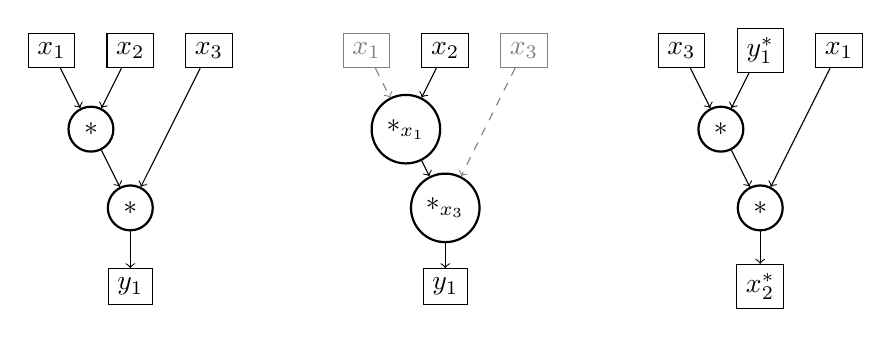
\begin{tikzpicture}
      \tikzstyle{node}=[circle,thick,draw=black,minimum size=4mm]
      \tikzstyle{arg}=[rectangle,thin,draw=black,minimum size=4mm]
      \tikzstyle{nodeg}=[circle,thick,draw=gray,minimum size=4mm]
      \tikzstyle{argg}=[rectangle,thin,draw=gray,minimum size=4mm]
      
      \begin{scope}
        \node[arg](in1){$x_1$};
        \node[arg,right of=in1](in2){$x_2$};
        \node[arg,right of=in2](in3){$x_3$};
        \node[node,below of=in1,xshift=5mm](times1){$*$};
        \node[node,below of=times1,xshift=5mm](times2){$*$};
        \node[arg,below of=times2](out){$y_1$};
        
        \path[->]
        (in1) edge (times1)
        (in2) edge (times1)
        (times1) edge (times2)
        (in3) edge (times2)
        (times2) edge (out);
      \end{scope}
      
      \begin{scope}[xshift=4cm]
        \node[argg](in1){\color{gray}{$x_1$}};
        \node[arg,right of=in1](in2){$x_2$};
        \node[argg,right of=in2](in3){\color{gray}{$x_3$}};
        \node[node,below of=in1,xshift=5mm](times1){$*_{x_1}$};
        \node[node,below of=times1,xshift=5mm](times2){$*_{x_3}$};
        \node[arg,below of=times2](out){$y_1$};
        
        \path[->]
        (in2) edge (times1)
        (times1) edge (times2)
        (times2) edge (out);
        
        \path[->,draw=gray,dashed]
        (in1) edge (times1)
        (in3) edge (times2);
      \end{scope}
      
      \begin{scope}[xshift=8cm]
        \node[arg](in1){$x_3$};
        \node[arg,right of=in1](in2){$y_1^\ast$};
        \node[arg,right of=in2](in3){$x_1$};
        \node[node,below of=in1,xshift=5mm](times1){$*$};
        \node[node,below of=times1,xshift=5mm](times2){$*$};
        \node[arg,below of=times2](out){$x_2^\ast$};

        \path[->]
        (in2) edge (times1)
        (times1) edge (times2)
        (times2) edge (out)
        (in3) edge (times2)
        (in1) edge (times1);
      \end{scope}
    \end{tikzpicture}  
  \end{center}

  \begin{itemize}
  \item Almost anytime we want to transpose, we end-up
    \emph{linearising} a circuit with multiplication nodes.
  \item Other constructs such as \texttt{if} statements and
    \texttt{for} loops need to be linearised too.
  \item Can we automatically deduce any possible linearisation of a
    program?
  \item \alert{Type inference systems can help us}
  \end{itemize}
\end{frame}

%%

\begin{pictureframe}
  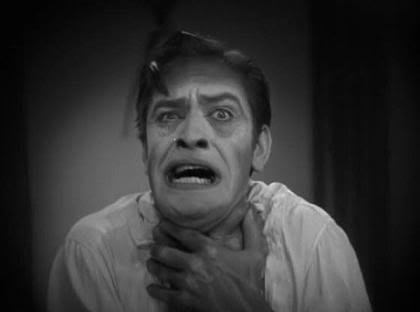
\includegraphics[width=\textwidth]{jekyll}
\end{pictureframe}

%%

\begin{frame}[fragile]
  \frametitle{Linearity inference}

  \begin{center}
    Suppose given a type \lstinline{R} implementing a ring. We want to
    define types \alert{\lstinline{L}} (for \emph{linear}) and
    \alert{\lstinline{S}} (for \emph{scalar}) such that the following
      equations hold
  \end{center}
  
  \begin{columns}
    \begin{column}{0.5\textwidth}
  \begin{semiverbatim}
    plus :: L -> L -> L
    plus :: S -> S -> S
  \end{semiverbatim}
    \end{column}
    \begin{column}{0.5\textwidth}
      \uncover<2>{\[\forall
        \alpha\in\{L,S\}.\alpha\ra\alpha\ra\alpha\]}
    \end{column}
  \end{columns}
  
  \begin{columns}[c]
    \begin{column}{0.5\textwidth}
  \begin{semiverbatim}
    times :: L -> S -> L
    \alt<2>{\st{times :: S {} -> L {} -> L}}{times :: S -> L -> L}
    times :: S -> S -> S
  \end{semiverbatim}
    \end{column}
    \begin{column}{0.5\textwidth}
      \uncover<2>{\[\forall
        \alpha\in\{L,S\}.\alpha\ra S\ra\alpha\]}
    \end{column}
  \end{columns}

  \begin{columns}
    \begin{column}{0.5\textwidth}
  \begin{semiverbatim}
    zero :: L
    zero :: S
  \end{semiverbatim}
    \end{column}
    \begin{column}{0.5\textwidth}
      \uncover<2>{\[\forall
        \alpha\in\{L,S\}.\alpha\]}      
    \end{column}
  \end{columns}

  \begin{columns}
    \begin{column}{0.5\textwidth}
  \begin{semiverbatim}
    one :: S
  \end{semiverbatim}
    \end{column}
    \begin{column}{0.5\textwidth}
    \end{column}
  \end{columns}
\end{frame}  

\begin{frame}[fragile]
  \frametitle{Linearity inference}
  
  \begin{center}
    The solution in Haskell
  \end{center}

  \begin{lstlisting}
    data L = L R
    data S = S R
    
    class Ring r where
      zero :: r
      (<+>) :: r -> r -> r
      neg :: r -> r
      (<*>) :: r -> S -> r

    one = S oneR
    (S a) == (S b) = a == b
  \end{lstlisting}

  \begin{center}
    To treat \alert{\lstinline{times :: S -> L -> L}}, we extend the
    Hindley-Milner type inference to handle lists of acceptable
    unifications.
  \end{center}
\end{frame}

%%
%%

\section{Automatic transposition}

\lstset{language=python}

\begin{frame}[fragile]
  \frametitle{\tALpy{}}

  \begin{block}{Algebraic types}
    \begin{itemize}
    \item \textbf{Prototypes}: {\tt Ring}, {\tt Module}, (optionally
      {\tt Algebra}, \dots)
    \item Declaring an algebraic type:
\begin{lstlisting}
  type Ring R
  type Module(R) M
\end{lstlisting}
    \end{itemize}
  \end{block}

  \begin{block}{Declaring a function}
\begin{lstlisting}
  def (linear M A, const m)f(linear M Z, const M z, n):
\end{lstlisting}
  \end{block}

  \begin{block}{Other constructs}
    \begin{itemize}
    \item Standard types ({\tt int}, {\tt bool}, \ldots)
    \item {\tt if}, {\tt for}, recursion, {\tt let} binding (assignment),
    \item Algebraic operators $+$, $\times$, projection/injection
      \verb|a[n]|.
    \end{itemize}
  \end{block}
\end{frame}

%%

\begin{frame}[fragile]
  \frametitle{Automatic transposition: the scalars first!}

\begin{semiverbatim}
  \textcolor{blue}{def} (linear R c)f(linear R a, const R \underline{b}):
    \underline{d} = \underline{b} * \underline{b}
    c = a * \underline{d}
\end{semiverbatim}

\begin{block}{}
  \centering
  \alt<1>{
    \begin{itemize}
    \item Run the algorithm backwards transposing each instruction.
    \end{itemize}
    
    \large \alert{Wrong!}
  }{
    \begin{itemize}
    \item First run the algorithm in the normal direction to compute
      all the scalar values,
    \item then run the algorithm backwards transposing each instruction.
    \end{itemize}
  }
\end{block}

\begin{semiverbatim}
  \textcolor{blue}{def} (linear R a)fT(linear R c, const R b):
    \only<2>{\textcolor{green}{# Forward sweep}
    \underline{d} = \underline{b} * \underline{b}

    \textcolor{green}{# Reverse sweep}
    }\alert<1>{a = c * \underline{d}}
    \only<1>{\underline{d} = \underline{b} * \underline{b}}
\end{semiverbatim}

\end{frame}

%%

\begin{frame}[fragile]
  \frametitle{Automatic transposition: \lstinline{if}'s and function calls}

\begin{lstlisting}
  def (linear M a)f(linear M b, n):
    if n > 0:
      a = f(b, n - 1)
      a[n] += R.Z(n) * b[n]
\end{lstlisting}

\begin{block}{}
  \begin{itemize}
  \item \lstinline{if}'s stay the same, the values appearing in the
    test \alert{must be scalar},
  \item (recursive) functions get their linear input and output
    parameters swapped, scalar arguments do not move.
  \end{itemize}
\end{block}

\begin{lstlisting}
  def (linear M b)fT(linear M a, n):
    # Reverse sweep
    if n > 0:
      b[n] += R.Z(n) * a[n]
      b += fT(a, n - 1)
\end{lstlisting}
  
\end{frame}

%%

\begin{frame}
  \frametitle{Scalar prediction and tail recursion}

  \begin{itemize}
  \item Permuting the order of the instructions may break tail/head
    recursion,
  \item this implies loss of efficiency,
  \item equivalently, in {\tt for} loops we have to precompute all the
    scalar values of the loop,
  \item \alert{this seems to increase the space requirements of the
      algorithm}, but does not affect the number of arithmetic operations.
  \end{itemize}
\end{frame}

%%

\begin{frame}[fragile]
  \frametitle{Lazy evaluation in the forward sweep}

  \begin{columns}
    \begin{column}{0.5\textwidth}
\begin{lstlisting}
def (R a, R b)f(R c, R d):
  if d > 0:
    x, y = f(c, d - 1)
    a, b = x * y, y + 1
  else:
    a, b = c, d
\end{lstlisting}
    \end{column}
    \begin{column}{0.5\textwidth}
\begin{lstlisting}
def (R c, R b)fT(R a, R d):
  # Forward sweep
  if (d > 0):
    _, y = f(a, d - 1)
    b = y + 1
  else:
    b = d
    
  # Reverse sweep
  if (d > 0):
    x = a * y
    c, y = fT(x, d - 1)
  else:
    c = a
\end{lstlisting}      
    \end{column}
  \end{columns}

  \pause 
  
  {\color{red}
  \begin{picture}(0,0)
    \thicklines
    \put(280,133){\oval(80,15)}
  \end{picture}}
\end{frame}

%%
%%


\section{Conclusion}

\begin{frame}
  \frametitle{Conclusion}
  
  \begin{block}{What we achieved}
    \begin{itemize}
    \item Transposition of multilinear/recursive code.
    \item An (almost complete) python implementation of transposition
      in the form of a compiler/interpreter.
    \item \tALpy{} can be easily used on top of CAS that have a python
      interface.
    \item Other CAS will be able to use \tALpy{} as we will add more
      languages to the output of the compiler (OCaml and Haskell look
      easy, C is somewhat harder).
    \end{itemize}
  \end{block}

  \begin{block}{Limitations}
    \begin{itemize}
    \item We trust the user not to introduce side effects.
    \item No formal proof of correctness... Do I trust my compiler?
    \item It would be nice to have types checked statically
      $\rightarrow$ Implementation as a Haskell extension?
    \end{itemize}
  \end{block}
\end{frame}

%%

\lstset{language=python}

\begin{frame}[fragile]
  \frametitle{Karatsuba in \tALpy}

\begin{lstlisting}
def (M c)karatsuba(M a, M b, n):
  if n == 1:
    tmp = M.zero()
    tmp[0] += a[0]*b[0]
    c = tmp
  elif n > 1:
    a0, a1 = split(a, n/2, n)
    b0, b1 = split(b, n/2, n)
    x0 = karatsuba(a0, b0, n/2)
    x2 = karatsuba(a1, b1, n - n/2)
    x1 = karatsuba((a1 + a0), (b1 + b0), n - n/2) - x0 - x2
    c = shift(x2, n, n+1) + shift(x1, n/2, n+1) + x0
\end{lstlisting}
\end{frame}

%%

\begin{frame}[fragile]
  \frametitle{Karatsuba in \tALpy}

  \lstset{basicstyle=\ttfamily\footnotesize}
\begin{lstlisting}
(M b)karatsubaT(M a, M c, n)
  # Forward sweep
  if (n == 1):
    pass
  elif n > 1:
    a0, a1 = split(a, n / 2, n)
  # Reverse sweep
  if (n == 1):
    tmp = c
    _transAL_tmp_0[0] += a[0] * tmp[0]
    b = _transAL_tmp_0
  elif n > 1:
    x2 = trans shift(c, n, n + 1)
    x1 = trans shift(c, n / 2, n + 1)
    x0 = c
    b1 = trans karatsuba(x1, a1 + a0, n - n / 2)
    b0 = b1
    x0 += - x1
    x2 += - x1
    b1 += trans karatsuba(x2, a1, n - n / 2)
    b0 += trans karatsuba(x0, a0, n / 2)
    b = trans split(b0, b1, n / 2, n)
\end{lstlisting}
\end{frame}

%%
%%

\section{Categories}

\begin{pictureframe}
  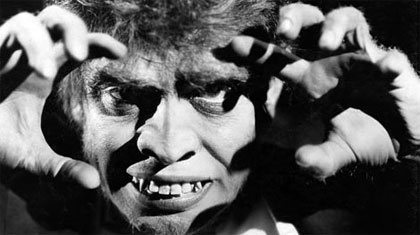
\includegraphics[width=\textwidth]{hyde2}
\end{pictureframe}

%%

\begin{frame}[fragile]
  \frametitle{Proof of the transposition theorem}

  \begin{columns}
    \begin{column}{0.5\textwidth}
      \begin{center}
        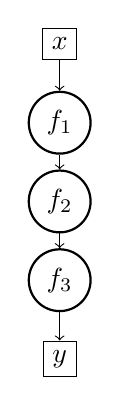
\begin{tikzpicture}
          \tikzstyle{node}=[circle,thick,draw=black,minimum size=4mm]
          \tikzstyle{arg}=[rectangle,thin,draw=black,minimum size=4mm]
          
          \begin{scope}
            \node[arg](x1){$x$};
            \node[node](x2)[below of=x1]{$f_1$};
            \node[node](x3)[below of=x2]{$f_2$};
            \node[node](x4)[below of=x3]{$f_3$};
            \node[arg](x5)[below of=x4]{$y$};
            
            \path[->]
            (x1) edge (x2)
            (x2) edge (x3)
            (x3) edge (x4)
            (x4) edge (x5);
          \end{scope}
        \end{tikzpicture}
      \end{center}
    \end{column}
    \begin{column}{0.5\textwidth}
      \only<2>{
        \[ \xymatrix{
          A \ar[d]^{f_1}\\
          A \ar[d]^{f_2}\\
          A \ar[d]^{f_3}\\
          A
        }\]}
      \only<3>{
        \[\xymatrix{
          & A \ar[dl]_{f_1} \ar[dr]^{g_1}\\
          A \ar[d]_{f_2} && A\ar[d]^{g_2}\\
          A \ar[dr]_{f_3} && A\ar[dl]^{g_3}\\
          & A
        }\]
      }
    \end{column}
  \end{columns}      

  \begin{center}
    \[(M_{f_1}M_{f_2}\cdots M_{f_n})^T = M_{f_n}^T\cdots M_{f_2}^TM_{f_1}^T\]

    \large
    \uncover<2->{Transposition is a contravariant functor}
  \end{center}
\end{frame}

%%

\begin{frame}
  \frametitle{Categorical semantics}

  \begin{itemize}
  \item Diagrams have a \emph{semantic} in any category,
  \item Circuits have a \emph{semantic} in any Cartesian category.
  \end{itemize}

  \begin{center}
    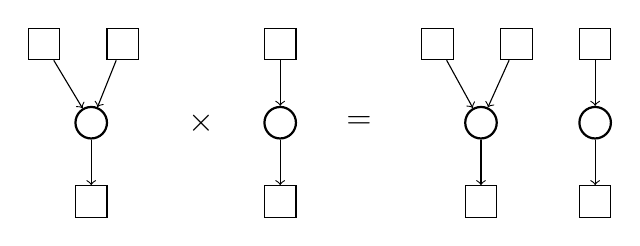
\begin{tikzpicture}
      \tikzstyle{node}=[circle,thick,draw=black,minimum size=4mm]
      \tikzstyle{arg}=[rectangle,thin,draw=black,minimum size=4mm]
          
      \begin{scope}
        \node[arg](x1){};
        \node[arg](x2)[right of=x1]{};

        \node[node](f)[below of=x1,xshift=6mm]{};

        \node[arg](x3)[below of=f]{};
        
        \path[->]
        (x1) edge (f)
        (x2) edge (f)
        (f) edge (x3);
      \end{scope}

      \begin{scope}[xshift=2cm,yshift=-1cm]
        \node(x){\large $\times$};
      \end{scope}

      \begin{scope}[xshift=3cm]
        \node[arg](x1){};

        \node[node](f)[below of=x1]{};

        \node[arg](x3)[below of=f]{};
        
        \path[->]
        (x1) edge (f)
        (f) edge (x3);
      \end{scope}

      \begin{scope}[xshift=4cm,yshift=-1cm]
        \node(x){\large $=$};
      \end{scope}

      \begin{scope}[xshift=5cm]
        \node[arg](x1){};
        \node[arg](x2)[right of=x1]{};
        \node[arg](x3)[right of=x2]{};

        \node[node](f1)[below of=x1,xshift=5.5mm]{};
        \node[node](f2)[below of=x3]{};

        \node[arg](x4)[below of=f1]{};
        \node[arg](x5)[below of=f2]{};
        
        \path[->]
        (x1) edge (f1)
        (x2) edge (f1)
        (x3) edge (f2)
        (f1) edge (x4)
        (f2) edge (x5);
      \end{scope}
    \end{tikzpicture}
  \end{center}

  \begin{itemize}
  \item Haskell's \lstinline{Control.Arrow} calls this operation
    \alert{\lstinline{***}},
  \item \lstinline{Control.Arrow} also gives \alert{\lstinline{&&&}},
    which is akin to our \alert{H} port.
  \end{itemize}
\end{frame}

%%

\begin{frame}
  \frametitle{Semantics and cosemantics}

  \begin{itemize}
  \item Transposition is just applying the functor to circuits
    (diagrams).
  \item But, wait a minute, transposition is \alert{contravariant}
    (and continuous and cocontinuous)!
  \end{itemize}

  {\large\[\prod \;\overset{?}{=}\; \coprod\]}

  \begin{itemize}
  \item Not in general: circuits have another \emph{semantic} in any
    Cocartesian category. Call it \emph{cosemantic}.
  \end{itemize}
  
  \begin{center}
    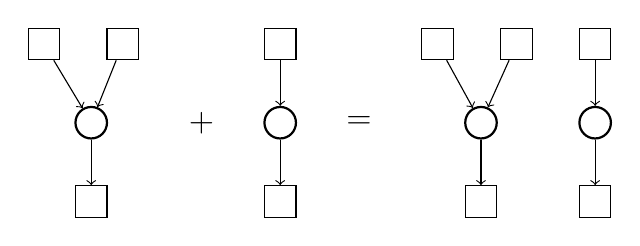
\begin{tikzpicture}
      \tikzstyle{node}=[circle,thick,draw=black,minimum size=4mm]
      \tikzstyle{arg}=[rectangle,thin,draw=black,minimum size=4mm]
          
      \begin{scope}
        \node[arg](x1){};
        \node[arg](x2)[right of=x1]{};

        \node[node](f)[below of=x1,xshift=6mm]{};

        \node[arg](x3)[below of=f]{};
        
        \path[->]
        (x1) edge (f)
        (x2) edge (f)
        (f) edge (x3);
      \end{scope}

      \begin{scope}[xshift=2cm,yshift=-1cm]
        \node(x){\large $+$};
      \end{scope}

      \begin{scope}[xshift=3cm]
        \node[arg](x1){};

        \node[node](f)[below of=x1]{};

        \node[arg](x3)[below of=f]{};
        
        \path[->]
        (x1) edge (f)
        (f) edge (x3);
      \end{scope}

      \begin{scope}[xshift=4cm,yshift=-1cm]
        \node(x){\large $=$};
      \end{scope}

      \begin{scope}[xshift=5cm]
        \node[arg](x1){};
        \node[arg](x2)[right of=x1]{};
        \node[arg](x3)[right of=x2]{};

        \node[node](f1)[below of=x1,xshift=5.5mm]{};
        \node[node](f2)[below of=x3]{};

        \node[arg](x4)[below of=f1]{};
        \node[arg](x5)[below of=f2]{};
        
        \path[->]
        (x1) edge (f1)
        (x2) edge (f1)
        (x3) edge (f2)
        (f1) edge (x4)
        (f2) edge (x5);
      \end{scope}
    \end{tikzpicture}
  \end{center}

  \begin{itemize}
  \item Haskell's \lstinline{ArrowChoice} calls this operation
    \alert{\lstinline{+++}}.
  \item \lstinline{ArrowChoice} also gives \alert{\lstinline{|||}},
    which is akin to our \alert{$+$} port.
  \end{itemize}
\end{frame}

%%

\lstset{basicstyle=\ttfamily\small}
\lstset{language=Haskell}

\begin{frame}[fragile]
  \frametitle{Additive categories}

  \begin{center}
    \large
    But $R\mathbf{-Mod}$ is an \alert{additive} category:

    $\quad\times\simeq+\quad\Rightarrow\quad$ cosemantic $\simeq$
    semantic
  \end{center}

  \begin{block}{Can we implement a type class synthesising these properties?}
\begin{lstlisting}
class AdditiveArrow (~>) where
  (&&&) :: (a ~> b) -> (a ~> c) -> (a ~> (Plus b c))
  (|||) :: (a ~> c) -> (b ~> c) -> ((Plus a b) ~> c)
  (***) :: (a ~> b) -> (c ~> d) -> ((Plus a c) ~> (Plus b d))
\end{lstlisting}
  \end{block}

  \pause
  
  \begin{center}
    \Large
    We tried, but we failed!

    \normalsize (this is essentially due to the limited support for
    dependent types in Haskell)
  \end{center}
  
\end{frame}

%%

\begin{frame}
  \frametitle{Future work}

  \begin{itemize}
  \item Earn Mr. Jekyll a doctoral degree.
  \item Finish the implementation of \tALpy{} and release it at
    \url{http://transalpyne.gforge.inria.fr/}.
  \item Write \lstinline{AdditiveArrow} in CoqMT.
  \end{itemize}
\end{frame}

%%
%%


{
  \setbeamertemplate{navigation symbols}{}
  \setbeamertemplate{background canvas}{
\includegraphics[width=\paperwidth]{hyde}}
  \begin{frame}[plain]
    \vspace{8cm}
    \begin{center}
      \textcolor{white}{\Huge The End?}
    \end{center}
  \end{frame}
}

%%
%%

\begin{frame}
  \frametitle{Bibliography}

  \begin{thebibliography}{1}
    
  \bibitem[Baur, Strassen '83]{BS83}
    W.~Baur and V.Strassen.
    \newblock The complexity of computing partial derivatives.
    \newblock \emph{Theoretical Computer Science} 22, pp. 317--330, 1983.

  \bibitem[Bordewijk '56]{Bor56}
    J.~L.~Bordewijk.
    \newblock Inter-reciprocity applied to electrical networks
    \newblock \emph{Applied Scientific Research B: Electrophysics, Acoustics, Optics, Mathematical Methods} 6, pages 1--74, 1956.

  \bibitem[Bostan, Lercerf, Schost '03]{BLS03}A.~Bostan, G.~Lecerf \& E.~Schost,
    \newblock Tellegen's Principle into Practice.
    \newblock \emph{Proceedings of ISAAC 2003}.

  \bibitem[B\"urgisser, Clausen, Shokrollahi]{BCS}P.~Bürgisser, M.~Clausen \& M.~A.~Shokrollahi,
    \newblock \emph{Algebraic Complexity Theory}.
    \newblock Springer, 1997.

  \bibitem[D.F., Schost '09]{DFS09}
    L.~De~Feo and {\'E}.~Schost.
    \newblock Fast arithmetics in Artin-Schreier towers over finite fields. 
    \newblock In \emph{ISSAC'09}, pages 127--134. ACM, 2010.

  \end{thebibliography}
\end{frame}

\begin{frame}
  \frametitle{Bibliography}

  \begin{thebibliography}{1}
  
  \bibitem[Fiduccia '73]{Fid73}
    C.~M.~Fiduccia.
    \newblock \emph{On the algebraic complexity of matrix multiplication}
    \newblock PhD Thesis, Brown University, 1973.

  \bibitem[Hopcroft, Musinski '73]{HoMu73}
    J.~Hopcroft and J.~Musinski.
    \newblock Duality applied to the complexity of matrix multiplication
    and other bilinear forms.
    \newblock \emph{SIAM Journal on Computing}, vol. 2, pp. 159–173, 1973.
 
  \bibitem[Page, Brin, Motwani, Winograd '99]{google}
    L.~Page, S.~Brin, R.~Motwani and T.~Winograd.
    \newblock The PageRank Citation Ranking: Bringing Order to the Web.
    \newblock \emph{Technical Report}, Stanford InfoLab, 1999,
    \url{http://ilpubs.stanford.edu:8090/422/}.

  \bibitem[Shoup '95]{Sho95}
    V.~Shoup.
    \newblock A new polynomial factorization algorithm and its implementation.
    \newblock \emph{J. Symb. Comp.}, 20(4):363--397, 1995.
    
  \bibitem[Wiedemann '86]{Wie86}
    D.~H.~Wiedemann.
    \newblock Solving Sparse Linear Equations Over Finite Fields.
    \newblock \emph{IEEE Trans. Inf. Theory}, vol. IT-32:54--62, 1986.

  \end{thebibliography}
\end{frame}

\end{document}





%%% Local Variables: 
%%% mode:flyspell
%%% ispell-local-dictionary:"british"
%%% mode: TeX-PDF
%%% TeX-master: t
%%% End: 
%
% LocalWords:  Tellegen